\section{Installazione ed esecuzione}
Il codice relativo alla Product Baseline lo si può trovare al seguente link:
\begin{center}
	\url{linkAllaRepo}
\end{center}
Una volta fatto il clone della repository o dopo aver scaricato lo zip, sono necessari i seguenti passi per far partire l'applicazione:
\begin{enumerate}
	\item Posizionarsi nella root della repo ed eseguire nella shell:
		\begin{lstlisting}
	npm install -g ganache-cli
	npm install -g truffle
	npm i
		\end{lstlisting}
	\item In seguito sempre nella shell:
		\begin{lstlisting}
	./startBlockchain.ps1
		\end{lstlisting}
	\item Infine è necessario eseguire:
		\begin{lstlisting}
	./loadProject.ps1
		\end{lstlisting}
\end{enumerate}

A questo punto noterai che il tuo browser predefinito ha aperto automaticamente l'homepage.
Ora dovrai connetteri a Metamask: nel tuo browser clicca sull'icona di Metamask e accetta l'informativa sulla privacy e le condizioni d'uso. Poi clicca su \textbf{Main Network} e scegli \textbf{Custom RPC}, inserisci nel primo form \textbf{http://localhost:9545} come in Figura~\ref{fig:metamask1} e clicca su  \textbf{Save}.
%Now you have to connect MetaMask: in your browser click on the MetaMask icon and accept the Privacy Notice and the Terms of use. Then click on \textbf{Main Network} and choose \textbf{Custom RPC}, type in the first form \textbf{http://localhost:9545} as in Figure~\ref{fig:metamask1} and click \textbf{Save}.

\begin{figure}[h]
\centering
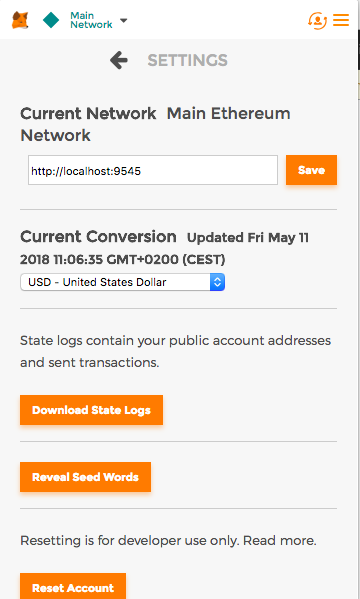
\includegraphics[height=3in]{./img/settings.png}
\caption{Setta l'RPC inserendo \textbf{http://localhost:9545}}
\label{fig:metamask1}
\end{figure}

Ora, come in Figura~\ref{fig:metamask2}, clicca su \textbf{Import Existing DEN} e (vedi Figura~\ref{fig:metamask3}) inserisci la frase \textbf{candy maple cake sugar pudding cream honey rich smooth crumble sweet treat} e la password che vuoi usare per il tuo account.


\begin{figure}[h]
\centering
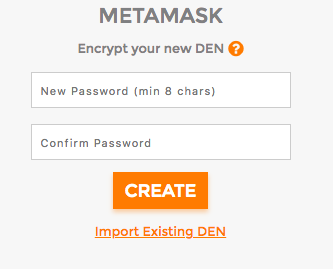
\includegraphics[height=1.8in]{./img/importa.png}
\caption{Clicca su \textbf{Import Existing DEN}}
\label{fig:metamask2}
\end{figure}

\begin{figure}[h]
\centering
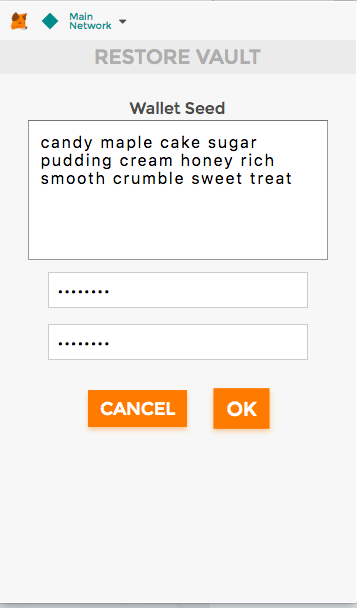
\includegraphics[height=3in]{./img/stringa_psw.png}
\caption{Inserisci la seed phrase e la password che vuoi usare}
\label{fig:metamask3}
\end{figure}



\clearpage